%  !TeX  root  =  user_guide.tex 

%\subsection{Quick Print Plugin}
\section{Extension Impression Rapide}\label{quickprint}

% when the revision of a section has been finalized, 
% comment out the following line:
% \updatedisclaimer

%The \toolbtntwo{quick_print}{Quick Print} Plugin makes it possible to export the current 
%map canvas to PDF format quickly and easily, with minimal effort. The only parameters that 
%need to be specified are a Map Title, a Map Name, and the Paper Size (See Figure~\ref{fig:quickprint}). 
%If you require additional control over the map layout, 
%please use the print composer plugin, described in Section~\ref{label_printcomposer}.
L'extension \toolbtntwo{quick_print}{Impression Rapide} permet d'exporter rapidement, facilement et avec un minimum d'effort l'emprise de la carte courante au format PDF. Les seuls paramètres devant être spécifiés sont le titre  de la carte, le nom de la carte et la taille de la page (voir la Figure~\ref{fig:quickprint}).  Si vous avez besoin de procéder à des réglages supplémentaires sur la mise en  page de carte, il vous est recommandé d'utiliser plutôt la fonction de composition de carte, décrite dans la Section~\ref{label_printcomposer}.

%\begin{figure}[ht]
%   \begin{center}
%   \caption{Quick Print Dialog \nixcaption}\label{fig:quickprint}\smallskip
%   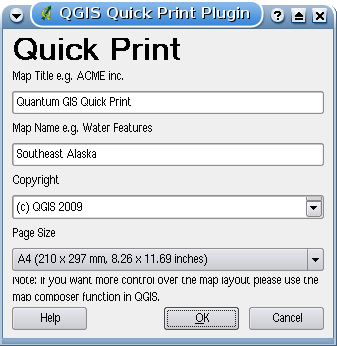
\includegraphics[clip=true, width=6cm]{quick_print_dialog}
%\end{center}
%\end{figure}
\begin{figure}[htb]
\centering
   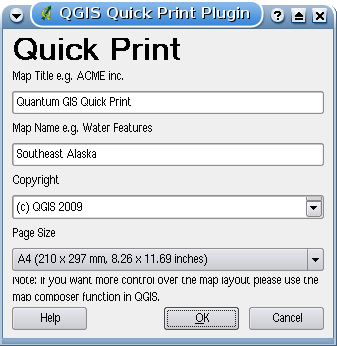
\includegraphics[clip=true, width=5cm]{quick_print_dialog}
 \caption{Boîte de dialogue de l'Impression Rapide \nixcaption}\label{fig:quickprint}
\end{figure}

%\begin{figure}[ht]
%   \begin{center}
%   \caption{Quick Print result as DIN A4 PDF using the alaska sample dataset\nixcaption}\label{fig:quickprint_result}\smallskip
%   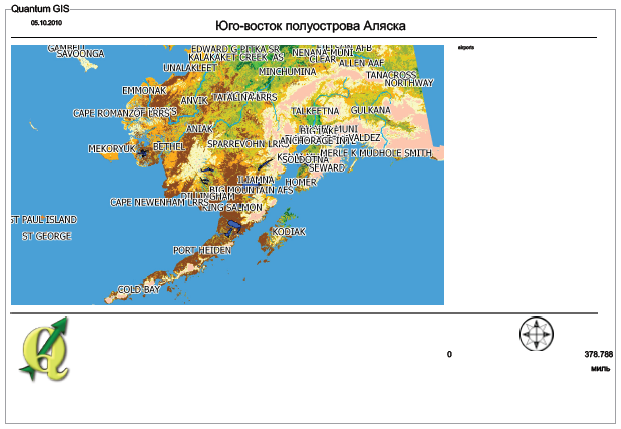
\includegraphics[clip=true, width=9cm]{quick_print_result}
%\end{center}
%\end{figure}
\begin{figure}[htb]
\centering
   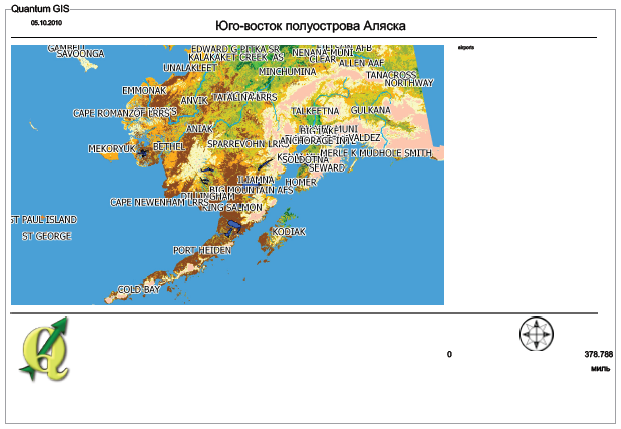
\includegraphics[clip=true, width=9cm]{quick_print_result}
   \caption{Résultat d'Impression Rapide au format PDF A4 DIN réalisé sur 
   l'échantillon de données de l'Alaska\nixcaption}\label{fig:quickprint_result}
\end{figure}
